\chapter{Stochastic Approximation}
%
Having completed the components for preserving the correct equilibrium distribution, I now turn to the task of developing the on-line adaptation scheme for biasing toward states with desirable free energy properties.
%
In order to do this, I turn to stochastic approximation, which has been used successfully in many contexts, especially Monte Carlo~\cite{Robbins1951, Tan2017,Liang2007, Park2006}.
%
\section{Stochastic Approximation for Molecular Simulation}
%
Before deriving the update rule for the present case, I will briefly review applications of stochastic approximation in molecular simulation.
%
Often, when one is simulating from an expanded ensemble, the mixture components (individual discrete states) will have very different free energies.
%
Since the relative population is given by
\begin{equation}
    \frac{p(k=n)}{p(k=m)} = e^{- \beta (\Delta G_n -\Delta G_m)}
\end{equation}
\noindent even small differences in free energies will result in very large differences in relative populations.
%
Practically speaking, this results in only rarely calculating acceptance probabilities between certain states, and therefore poor statistics in the final estimate of relative free energies.
%
To resolve this, one approach is to attempt to flatten the histogram of states.
%
In order to achieve this flattening, one could use the expanded ensemble weights $g_k$ add additional weight to those states with a lower free energy.
%
This requires knowing the relative free energies, however, defeating the purpose of running the algorithm in the first place.
%
Therefore, many adaptive schemes have been developed to estimate these weights online, such as in \cite{Wang2001} \cite{Tan2017} \cite{Liang2007}.
%
\subsection{SAMS}
%
Recently, a formulation of stochastic approximation Monte Carlo was developed by Tan \cite{Tan2017} that is asymptotically optimal in the sense of minimizing the variance of the weights $g_k$.
%
This algorithm is performed as follows:
%
\begin{eqnarray} \label{binary-sams-sa}
     g^{(t-1/2)}_k = g^{(t-1)}_k - t^{-1} \frac{\delta_{s_t,k}}{\pi_k} \\
     g^{(t)}_k = g^{(t-1/2)} - g^{(t-1/2)}_1
\end{eqnarray}
%
\noindent where each $g^{(t)}_k$ is the adapted weight of chemical state $k$ at iteration $t$, $s_t$ is the current state at iteration $t$, and $\pi_k$ is the target probability for state $k$.
%
Setting each $\pi_k = \frac{1}{n}$ for a system with $n$ states will result in even sampling, and asymptotically will result in weights equal to the relative free energies \cite{Tan2017}.
%
%
Its simplicity, combined with its asymptotic optimality~\cite{Tan2017}, makes it an appealing choice for adaptively reweighting the components of the expanded ensemble.
%
Although this can be very useful for determining the entire set of pairwise relative free energies, it can still be very burdensome for large sets of chemical states.
%
In general, we are not interested in merely even sampling, as we are not concerned with the relative free energies of two unfavorable chemical states.
%
Therefore, we seek an adaptive algorithm that provides for greater sampling of chemical states that are favorable according to some free energy criterion.
%
\section{Doubly-recursive SAMS}
%
In general, in physical simulation tasks, we seek states that optimize a free energy difference between multiple states, not simply a single state.
%
For instance, if we are optimizing to maximize binding affinity, the quantity we seek to maximize is (omitting constants) the association constant $K_a$:
%
\begin{equation}
    K_a \propto \frac{Z_{PL}}{Z_{P}Z_{L}}
\end{equation}
%
\noindent where $Z_*$ represents the normalizing constant of the appropriate species $*$, $P$ and $L$ represent protein in solvent and ligand in solvent systems respectively, and $PL$ represents the interacting protein-ligand complex system.
%
Since we are trying to find the chemical state which maximizes this quantity, we are generally interested in so-called relative free energies.
%
As a result, when comparing two ligands, $L_1$ and $L_2$, we have:
\begin{eqnarray}
     K_{a,1} &=& \frac{Z_{PL_1}}{Z_{P}Z_{L_1}} \\
     K_{a,2} &=& \frac{Z_{PL_2}}{Z_{P}Z_{L_2}} \\
     K_{relative} &=& \frac{K_{a,1}}{K_{a,2}} = \frac{\frac{Z_{PL_1}}{Z_{P}Z_{L_1}}}{\frac{Z_{PL_2}}{Z_{P}Z_{L_2}}} = \frac{\frac{Z_{PL_1}}{Z_{L_1}}}{\frac{Z_{PL_2}}{Z_{L_2}}} = \frac{Z_{PL_1}}{Z_{PL_2}} \frac{Z_{L_2}}{Z_{L_1}}
\end{eqnarray}
%
\noindent Therefore, if we would like a chemical state to be sampled according to its relative binding affinity, we need to adapt the weights of the chemical states such that
%
\begin{equation}
    p(k) \propto \frac{Z_{PL_k}}{Z_{L_k}}
\end{equation}
%
That is, the target weights $\pi$ must be adapted as well, since we do not know \emph{a priori} what the relative free energies are.
%
\subsection{Description of Algorithm}
%
More generally, consider we have $s$ different probability densities:
%
\begin{eqnarray}
p_{ij}(x) &=& e^{g_{ij}^*} q_{ij}(x) \:\:,\:\: i = 1,\ldots, s\:\:, \:\: j = 1,\ldots, m
\end{eqnarray}
%
and we desire to design a chain where the marginal distributions of all $s$ chains are
%
\begin{eqnarray}
p_{ij} &\propto& \prod_{i'=1}^s e^{-\theta_s g_{i'j}^*} = \exp\left[ - \sum_{i'=1}^s \theta_s g_{i'j}^* \right] \forall i = 1,\ldots, s
\end{eqnarray}
%
where the \emph{design vector} $\Theta \equiv \{ \theta_1, \ldots, \theta_s \}$ specifies how different targets and antitargets are used in weighting the design constraints.
%
We postulate that we can do this by defining $\pi_i(Z)$ for $Z \equiv \{g_1, \ldots, g_s\}$ as
%
\begin{eqnarray}
p_{ij}(Z | \Theta) &\propto& \exp\left[ - \sum_{i'=1}^s \theta_s g_{i'j} \right]
\end{eqnarray}
%
\section{Toy Examples}
%
Having described the algorithm in principle, I now present a simple toy example to empirically see that the quantity of interest is generated.
%
In this example, we simulate a set of harmonic oscillators:
\begin{eqnarray}
    p_{i0} \propto e^{-\beta \frac{K_{i0}}{2} (x - x_{i0})^2} \\
    p_{i1} \propto e^{-\beta \frac{K_{i1}}{2} (x - x_{i1})^2}
\end{eqnarray}
%
As a model of the binding free energy calculation, we would like:
\begin{equation}
    p_{1}(k) \propto \frac{Z_{1_k}}{Z_{2_k}}
\end{equation}
%
\noindent where the subscripts 1 and 2 indicate the different chains (analogous to complex and solvent for the binding free energy).
%
\begin{figure}
    \centering
    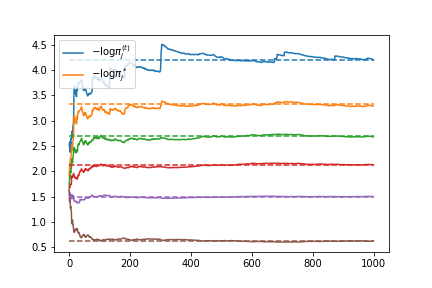
\includegraphics{logpitrace_s_nosep.png}
    \caption{The target weights of the various harmonic oscillators (solid) and the true value (dotted line). Note that the higher free energy states take significantly longer to converge to their true values}
    \label{fig:toy_doublesams}
\end{figure}
%
As can be seen in Figure~\ref{fig:toy_doublesams}, the target weights of the favorable states (lower free energy) converge faster.
%
This is what we desire, since we are not interested in how much more unfavorable one high free energy state is from another.
%
We can extend this principle to multiple chains as well; as generalized above, this applies to cases such as multitargeting (finding chemical states with a favorable free energy in multiple chains) or selectivity (finding states that are favorable for one but not another). 
%
\subsection{Performance}
%
Ultimately, the goal of the algorithm is to more quickly explore relevant regions of chemical space.
%
However, there are some limitations to the stochastic approximation algorithm presented here that are worth discussion.
%
\section{Limitations}
%
Two issues arise when discussing the limitations of the stochastic approximation algorithm used here.
%
The first is the convergence rate. Since the algorithm works by counting the numbr of times different states are visited, it can take a lengthy simulation before the chemical state space begins to be explored.
%
The second limitation is that the SA algorithm presented here is designed for a fixed number of states.
%
However, it is clear that to truly carry out molecular design, an algorithm must be capable of handling the situation where the number of states is not known \emph{a priori}.
%
This can arise, for instance, when the proposal distribution is a neural network.
%
\subsection{Convergence Rate}
%
The first topic of concern is the convergence rate.
%
To examine this in greater detail, we observe behavior in a toy model.
%
Even in the traditional binary SAMS update (described in \cite{Tan2017}), it can take many iterations to begin to achieve even sampling, especially if the mixture components are kinetically separated.
%
\begin{figure}
    \centering
    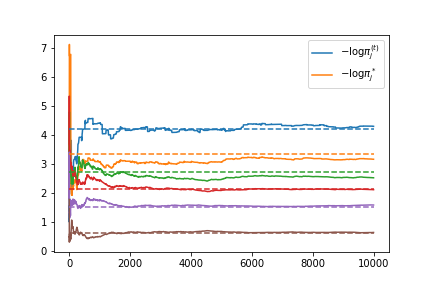
\includegraphics{logpitrace_s_smallsep.png}
    \caption{Convergence of binary SAMS from a single realization of harmonic oscillators with only a small separation in means.}
    \label{fig:smallsep}
\end{figure}
%
In Figure~\ref{fig:smallsep}, one can see that the desired target weights (dotted lines) are quickly approached by the adapted target weights (solid lines), and are more quickly approached for low free energy states than others.
%
However, what happens if we add a small amount of kinetic separation to these harmonic oscillators?
%
In principle, this issue is resolve by nonequilibrium switching; however, in practice, efficiently resolving these types of issues is quite difficult, especially when the states between which one must transition are so diverse.
%
More work needs to be performed to not only initialize the weights well, but investigate the possibility of initial algorithms that may approach the desired target more quickly than the asymptotic algorithm.
%
\subsection{Number of States}
%
Ideally, we'd be able to jump to new (unseen) chemical states, which would enable molecular design in a truer sense.
%
However, the formulation of the SA algorithm above clearly is designed for a fixed number of states.
%
One way to resolve this is to imagine that, although more states may be added on the fly, we set an upper limit on how many states can be explored.
%
In this case, we will eventually reach the maximum number of states, at which point the algorithm obviously becomes the double recursion SA above.
%
However, there are some questions regarding this.
%
We already saw that the convergence of the algorithm is highly sensitive to the mixing of the underlying sampler; what happens when the number of states changes?
%
This is a subject that calls for further investigation and future work.
%
\section{Weight initialization}
%
One major challenge with SAMS algorithms is how the weights are initialized.
%
The initial weights will have a profound effect on the performance, especially as weight adaptation diminishes.
%
For this reason, many use a multiple-stage scheme as in \cite{Tan2017}; this allows the weights to initially adapt much more quickly, and then revert to the asymptotically optimal gain decay after a certain condition is reached.
%
In addition to this scheme, it is advantageous to determine whether there exists simple tricks that can initialize the SAMS weights nearer the correct target than zero.
%
\subsection{Implicit volume term}
%
One issue that the reversible jump-based simulation incurs that most others do not is that the dimensionality of phase space changes with the chemical state.
%
As a result, depending on the units used, there is a volume term that is not accounted for in the acceptance probability.
%
Since in free energy calculations we are always looking at differences, this is not a concern for accuracy, but is for efficiency, since this term will cause certain states to become very unfavorable based on the number of degrees of freedom in that state.
%
Observing this discrepancy, I decided to initialize the stochastic approximation weights for each state using a very rough guess of the implicit volume term: 
%
\begin{eqnarray}
g_k^0 &=& n_{heavy}*4.5 + n_{hydrogen}*3.8
\end{eqnarray}
%
The hydrogen term is smaller because it only has two degrees of freedom (bonds are constrained).
%
\subsection{Hydration}
%
A common environment in relative free energy calculations is the solvent phase, which consists of just the small molecules in solvent.
%
Since the environment is essentially the same in solvent regardless of the target, it is advantageous to develop a quick initialization scheme that can be easily reused.
%
Here, I implemented one scheme, however, there exists the potential for other schemes to be developed as well.
%
\subsubsection{Initialize with minimized point energies}
%
One interesting approach for initializing weights in the solvent phase is to use the minimized point energies of the corresponding molecule in implicit solvent.
%
In \cite{mobley2008} this approach was explored as an approximation to the hydration free energy of the molecule.
%
Since we do not rely on the initialization of weights for correctness, only for efficiency, a simple scheme like this one is useful.
%
It is possible that more sophisticated implicit solvent models (such as PBSA~\cite{Tan2006}) would produce superior starting weights, but the added cost may not be justified.
%
%
\subsection{Complex weight initialization}
%
In molecular design problems relating to drug discovery, another common phase is the complex phase--that is, protein and ligand interacting in solvent.
%
This phase usually contains systems that have many more atoms, as well as much longer correlation times.
%
Therefore, it would be extremely helpful to have an efficient weight initialization scheme.
%
However, the complex phase poses several additional challenges.
%
One challenge is that the relative free energies of different chemical states in the complex phase cannot be as easily estimated as in the solvent phase.
%
Another is that the complex phase varies greatly between different projects; one cannot come up with a single, simple initialization scheme for all complex phase calculations as one can for the solvent phase.
%
However, there are several ideas that may be implemented.
%
%
\subsubsection{Initial acceptance probability}
%
One simple idea is to use the initial $\ln P_\mathrm{accept}$ values that are generated by the algorithm.
%
This is appealing intuitively, because $P_\mathrm{accept}$ is a (very poor) estimate of the relative free energy of the two states~\cite{Zwanzig1954}, as well as being produced as a byproduct of the algorithm (requiring no additional effort).
%
However, there are several pitfalls to this approach. 
%
In particular, due to the potentially high variance of the $P_\mathrm{accept}$, setting a stochastic approximation weight with it can result in an initialization extremely far from the true value.
%
This would actually make the simulation even less efficient.
%
One approach would be to only initialize the weight with the initial acceptance probability if the log acceptance probability is within some bounds.
%
This might prevent the SAMS weights from being initialized to quantities very far from the true value, while still allowing a decent initial guess.
%
%
\subsubsection{Machine learning score}
%
Another approach not explored here would involve using a machine learning algorithm that attempts to predict binding free energies~\cite{Colwell2018, Wu2018} to initialize the weights.
%
A caveat here would be that a machine learning algorithm that is more accurate or otherwise has a different error pattern than the forcefield might start the weights farther from the desired true values (even if they are more accurate in reality).
%
The area of weight initialization represents a fertile ground for future investigation.
%
\subsubsection{Implicit ligand theory}
%
Another interesting area of research is implicit ligand theory~\cite{Nguyen2018,Xie2017,Minh2012impl, Minharxiv}, which uses one or more snapshots of a rigid protein and simulates only the small molecule, resulting in an impressive speedup.
%
These rapidly-calculated approximations could be used to initialize the weights, providing a potentially profitable starting point.